\documentclass[a4paper,10pt]{article}
\usepackage[left=3cm,top=2cm,right=3cm,bottom=3cm,nohead]{geometry} %
\usepackage[utf8]{inputenc}
\usepackage{polski}
\usepackage{pbox}
\usepackage[table,xcdraw]{xcolor}
\usepackage{multirow}
\usepackage{tabularx}
\usepackage{amsmath}
\usepackage{pdfpages}
\usepackage{hyperref}
\usepackage{pgfplots}
\usepackage{placeins}
\usepackage{pgf}
\usepackage{tikz}
\usepackage{caption}
\usepackage{subfigure}
\usepackage{multicol}
\usepackage{xcolor}
\usepackage{listings}

\begin{document}
\definecolor{keywords}{RGB}{255,0,90}
\definecolor{comments}{RGB}{0,0,113}
\definecolor{red}{RGB}{160,0,0}
\definecolor{green}{RGB}{0,150,0}
 
\lstset{language=Python, 
    basicstyle=\ttfamily\small, 
    keywordstyle=\color{keywords},
    commentstyle=\color{comments},
    stringstyle=\color{red},
    showstringspaces=false,
    identifierstyle=\color{green},
}
% \renewcommand{\arraystretch}{1.8}
% \renewcommand{\arraystretch}{1.8}

\begin{titlepage}

\newcommand{\HRule}{\rule{\linewidth}{0.5mm}} % Defines a new command for the horizontal lines, change thickness here

\center % Center everything on the page
 
%----------------------------------------------------------------------------------------
%	HEADING SECTIONS
%----------------------------------------------------------------------------------------

\begin{center}\includegraphics[scale=0.6]{agh}\end{center}
\vspace*{10mm}
\textsc{\LARGE Akademia Górniczo-Hutnicza}\\[1.5cm] % Name of your university/college
\textsc{\Large Wydział Fizyki i Informatyki Stosowanej}\\[0.5cm] % Major heading such as course name
\textsc{\large Podstawy fizyki teoretycznej - laboratorium}\\[0.5cm] % Minor heading such as course title

%----------------------------------------------------------------------------------------
%	TITLE SECTION
%----------------------------------------------------------------------------------------

\HRule \\[0.4cm]
{ \huge \bfseries Zastosowanie metod dynamiki molekularnej dla gazu rzeczywistego}\\[0.4cm] % Title of your document
\HRule \\[1.5cm]
 
%----------------------------------------------------------------------------------------
%	AUTHOR SECTION
%----------------------------------------------------------------------------------------

% \begin{minipage}{0.4\textwidth}
% \begin{flushleft} \large
% \emph{Autorzy:}\\
% Karol Kozicki
% \end{flushleft}
% \end{minipage}
% ~
% \begin{minipage}{0.4\textwidth}
% \begin{flushright} \large
% \emph{Prowadzący:} \\
% dr inż. Piotr Kowalski
% \end{flushright}
% \end{minipage}\\[4cm]

% If you don't want a supervisor, uncomment the two lines below and remove the section above
\Large \emph{Autor:}\\
Karol \textsc{Kozicki}\\[3cm] % Your name

%----------------------------------------------------------------------------------------
%	DATE SECTION
%----------------------------------------------------------------------------------------

{\large \today}\\[3cm] % Date, change the \today to a set date if you want to be precise

%----------------------------------------------------------------------------------------
%	LOGO SECTION
%----------------------------------------------------------------------------------------

%\includegraphics{Logo}\\[1cm] % Include a department/university logo - this will require the graphicx package
 
%----------------------------------------------------------------------------------------

\vfill % Fill the rest of the page with whitespace


\end{titlepage}
\tableofcontents
\newpage
%------------------------------1-------------------------------
\begin{abstract}
Celem pracy jest jest przeprowadzenie symulacji dynamiki molekularnej gazu rzeczywistego odziałującego poprzez odziaływanie Lennarda-Jonesa. W pracy przedstawione są kolejno kroki niezbędne do uzyskania oprogramowania będącego w stanie symulować ruch cząstek a następnie przedstawione są wyniki tych symulacji. Określone zostały także makroskopowe parametry jakimi są temperatura oraz ciśnienie układu.
\end{abstract}

\section{Podstawy teoretyczne}

\subsection{Gaz rzeczywisty}
Gaz rzeczywisty jest to gaz który nie zachowuje się zgodnie z prawami którymi rządzi się gaz doskonały. W praktyce są to wszystkie gazy w przyrodzie bowiem model gazu doskonałego jest jedynie przybliżeniem lepiej lub gorzej działającym w zależności od parametrów opisujących układ.

\subsection{Potencjał Lennarda-Jonesa}

Potencjał Lennarda-Jonesa jest to jeden z rodzajów potencjałów odziaływania międzyatomowego. Jest to bardzo dobre przybliżenie dla gazów szlachetnych ale także sprawdza się dla innych atomów. Potencjał opisuje wzór:

\begin{equation}\label{eq:2}
U(r_{ij}) = 4\epsilon\left[\left(\frac{\sigma}{r_{ij}}\right)^{12} - \left(\frac{\sigma}{r_{ij}}\right)^6\right]
\end{equation}

gdzie:\\
$r_{ij}$ - jest odległością pomiędzy i-tym oraz j-tym atomem\\
$\sigma$ - parametr odległości zależny od pierwiastka\\
$\epsilon$ - parametr energii zależny od pierwiastka\\

Siłę działającą pomiędzy atomami możemy obliczyć z wzoru:

\begin{equation}\label{eq:3}
F = -\nabla U
\end{equation}

Powyższy potencjał w podanej formie został wykorzystany w implementacji.

\section{Przygotowanie do obliczeń}
\subsection{Wybrane oprogramowanie}
Wybrany jezyk programowania to $Python3$ \cite{python} który jest najlepszym wyborem z racji na swoją prostotę w tworzeniu kodu oraz jego przejrzystość. Aby wykonywane obliczenia były znacznie szybsze wykorzystana została biblioteka $NumPy$ wraz z biblioteką $SciPy$ do uzyskiwania rozkładów oraz stałych fizycznych.  Do graficznego przedstawienia wyników obliczeń numerycznych został wykorzystany program $Gnuplot$ \cite{gnuplot}, umożliwiający wykonywanie złożonych, w pełni dostosowanych wykresów w stosunkowo krótkim czasie.

\subsection{Warunki początkowe, stałe}
Przyjęte wartości będące stałymi przez cały okres symulacji wynoszą:

\begin{itemize}
\item Minimalny promień odcięcia (wytłumaczone w dalszej części) - $r_c = 0.25(0.3345 * 10^{-9})$
\item Promień odcięcia (wytłumaczone w dalszej części) - $r_c = 10r_c$
\item Wymiar pudła obliczeniowego - $dim(x) = dim(y) = dim(z) = 10^{-8}m$
\item Potencjał Lennarda-Jonesa - $\epsilon = 125.7 k_B$
\item Potencjał Lennarda-Jonesa - $\sigma = 0.3345 * 10^{-9}$
\item Masa cząstki $m = \frac{39.95 * 10^{-3}}{N_A}$ 
\end{itemize}

\section{Wyniki}

\subsection{Periodyczne warunki brzegowe}

Początkowo zaimplementowane zostały periodyczne warunki brzegowe. Implementacja polega na sprawdzaniu przy każdej iteracji czy pozycja cząstki nie wychodzi poza pudło symulacyjne o określonych z góry wymiarach. Jeśli któraś współrzędna cząstki przekracza odpowiadający wymiar, pozycja jest korygowana poprzez przeniesienie cząstki tak aby znajdowała się ponownie wewnątrz pudła.

Aby zweryfikować poprawność implementacji przeprowadzona została symulacja na jednej cząstce wewnątrz pudła z nadaną prędkością początkową (każda ze składowych prędkości ma inną wartość).

Poniżej przedstawione są wyniki symulacji w formie wykresów:

\begin{figure}[h]
\begin{center}
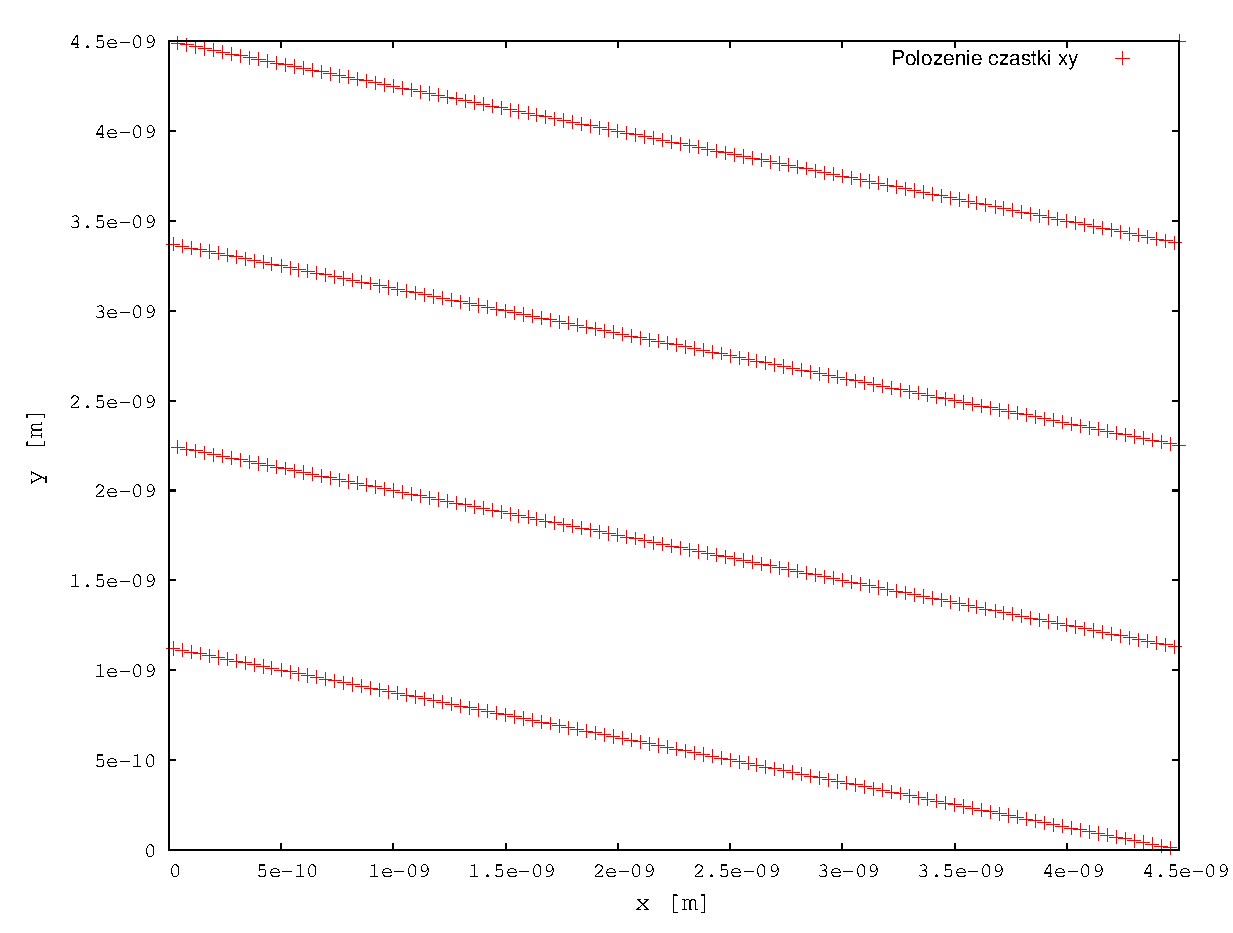
\includegraphics[scale=0.6]{wyniki/one-particle-xy.eps}
\caption{Pozycja cząstki wewnatrz pudła symulacyjnego w rzucie na płaszczyznę xy}
\label{pic:one-xy}
\end{center}
\end{figure}
\FloatBarrier

\begin{figure}[h]
\begin{center}
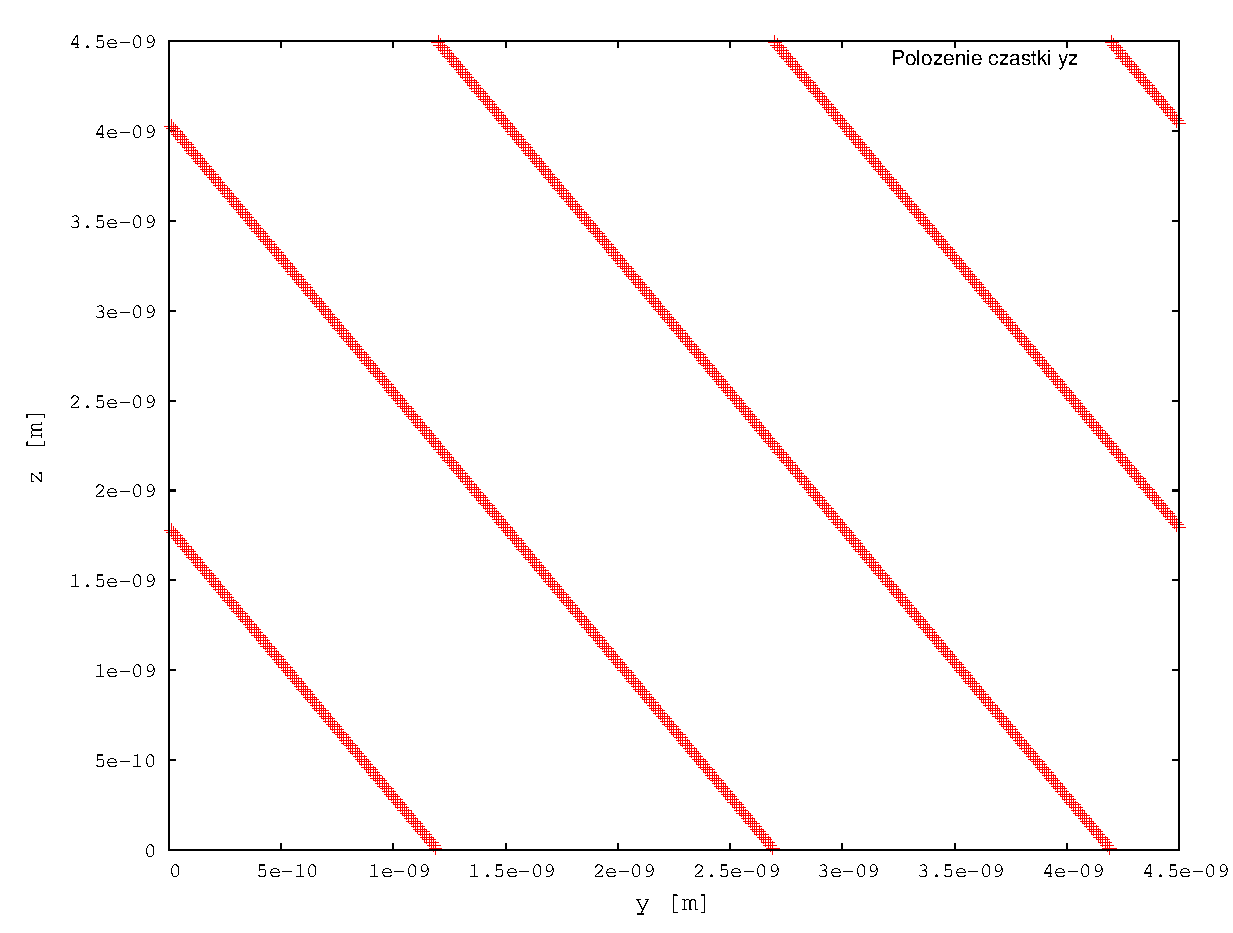
\includegraphics[scale=0.6]{wyniki/one-particle-yz.eps}
\caption{Pozycja cząstki wewnatrz pudła symulacyjnego w rzucie na płaszczyznę yz}
\label{pic:one-yz}
\end{center}
\end{figure}
\FloatBarrier

Z powyższych obrazków wnioskujemy, że implementacja periodycznych warunków brzegowych jest poprawna. Pozycja cząstki jest prawidłowo korygowana w każdym z wymiarów.

\subsection{Zderzenie dwóch cząstek}

Kolejnym krokiem była implementacja odziaływania cząstek. Zgodnie z wytycznymi zaimplementowano odziaływanie Lennarda Jonesa, jednak ogólność implementacji pozwala przeprowadzić symulację dla dowolnego typu odziaływania, należy jedynie wprowadzić odpowiednie stałe oraz relację energii od odległości.

Aby zweryfikować poprawność implementacji przeprowadzona została symulacja dwóch cząstek początkowo znajdujących się w dużej odległości pozwalającej zaniedbać początkową wartość energii potencjalnej. Prędkości cząstek zostały tak dobrane aby w relatywnie krótkim czasie nastąpiła kolizja tych cząstek.

Poniżej zaprezentowane są wyniki symulacji w formie wykresów:

\begin{figure}[h]
\begin{center}
\includegraphics[scale=0.6]{wyniki/2particles-collision.eps}
\caption{Zleżność energii kinetycznej, potencjalnej oraz całkowitej od czasu trwania symulacji}
\label{pic:collision}
\end{center}
\end{figure}
\FloatBarrier

\begin{figure}[h]
\begin{center}
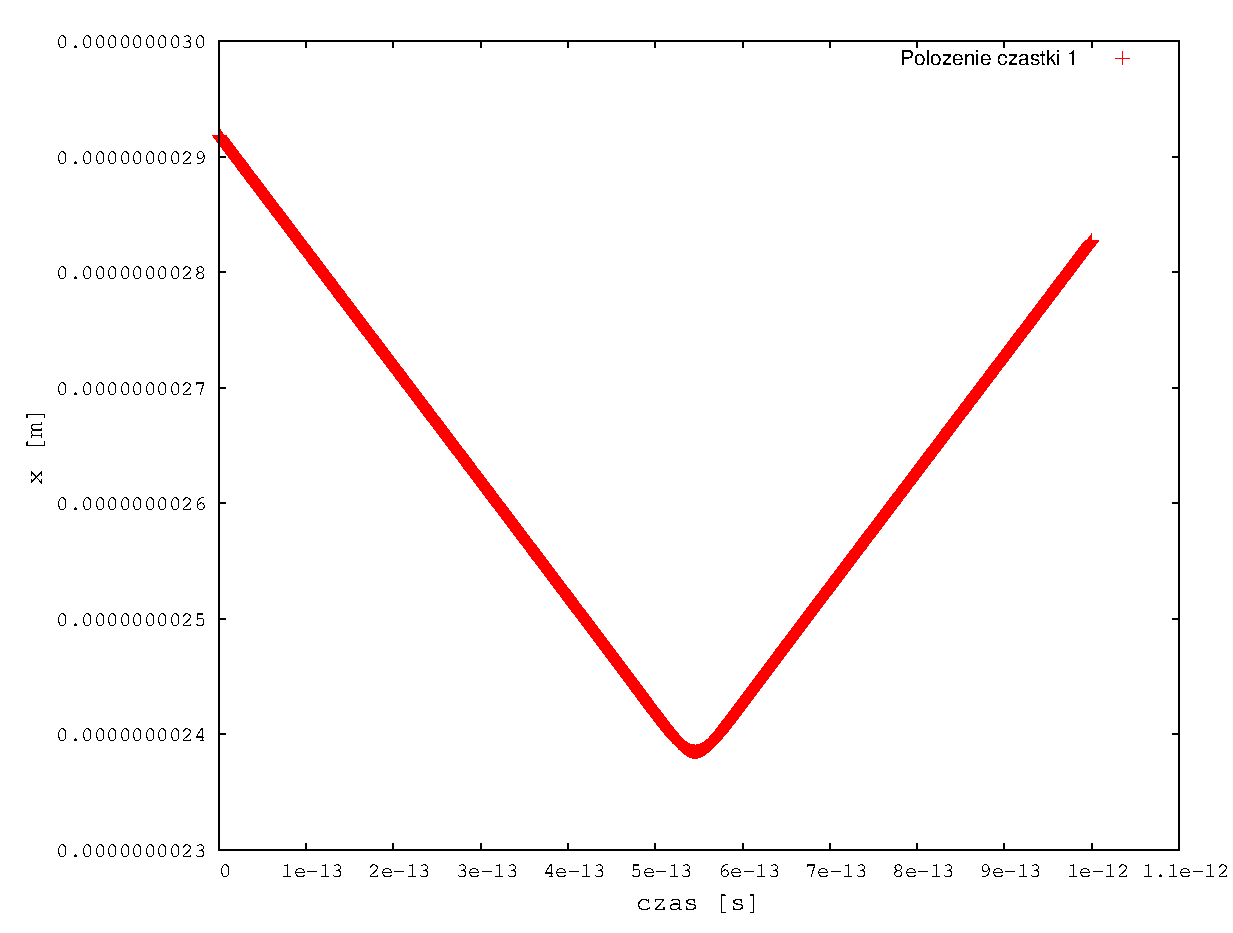
\includegraphics[scale=0.6]{wyniki/pos-particles-collision.eps}
\caption{Zleżność położenia (współrzędnej x) jednej z cząstek od czasu trwania symulacji}
\label{pic:collision-pos}
\end{center}
\end{figure}
\FloatBarrier

Z racji nie występowania żadnych zewnętrznych sił/potencjałów zdolnych zmieniać całkowitą energię układu, spodziewamy się stałości tego parametru. Symulacja zgadza się ze zdrowych rozsądkiem, mianowicie początkowo cząstka miała jedynie energię kinetyczną pochodzącą z niezerowej wartości początkowej prędkości każdej z cząstek. Gdy cząstki znajdują się w dostatecznie bliskiej odległości (jednak nie w bardzo bliskiej) następuje ich przyciąganie - jest to poprawnie opisany proces przez symulację. Widzimy narastanie energii kinetycznej oraz malenie energii potencjalnej. Następnie cząstki zbliżają się na odległość tak bliską, że zaczynają się odpychać. Proces ten poprawnie przedstawia symulacja, widzimy ostry spadek energii kinetycznej na koszt energii potencjalnej - energia ruchu zostaje zmagazynowana w energii potencjalnej odziaływania. Następnie cząstki zostają odepchnięte i ostatecznie poruszają się tak jak początkowo tylko w przeciwnym kierunku. W całym procesie odbicia energia całkowita jest zachowana co jest poprawnym zachowaniem. Oczywiście wartość ta fluktuuje jednak jest to fluktuacja spowodowana niezerowym krokiem czasowym.

\subsection{Obrazy cząstek}

Obrazy cząstki o położeniu $r_i$ są to wszystkie cząstki (wirtualne) w położeniach $r_i + R_n$, gdzie $R_n$ jest długością wymiaru pudła w n-tym wymiarze.

Z powodu wprowadzenia periodycznych warunków brzegowych w obliczeniach musimy brać pod uwagę także obrazy cząstek. Jest to niezbędny zabieg aby obliczenia były poprawne, ponieważ od odległości pomiędzy cząsteczkami zależy całkowita energia potencjalna.

Przy obliczeniach pod uwagę bierzemy najmniejszą z odległości pomiędzy i-tą cząstką a j-tą cząstką (lub jej obrazami). Konwencja ta nazywana jest konwencją minimalnego obrazu.

Aplikacja zawiera niezbędną implementację obrazów cząstek. Aby sprawdzić poprawność implementacji zasymulowano sytuację dwóch cząstek poruszających się naprzeciw siebie. Początkowa odległośc została dobrana tak aby odbicie następowało dokładnie na granicy pudła obliczeniowego.

Poniżej zaprezentowane są wyniki symulacji w formie wykresów:

\begin{figure}[h]
\begin{center}
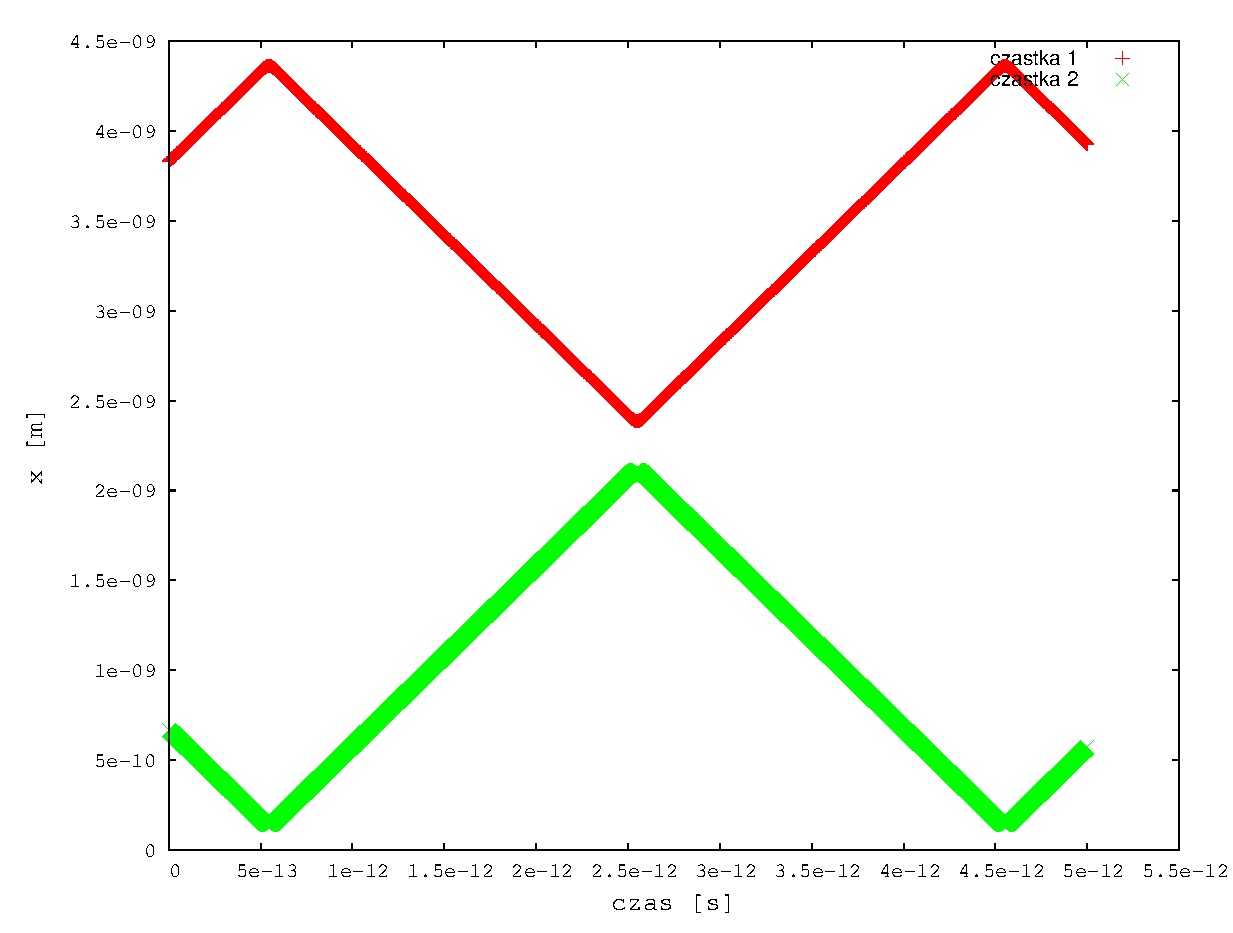
\includegraphics[scale=0.6]{wyniki/border-oscilating-particles2-pos.eps}
\caption{Położenie (współrzędna równoległa do prędkości) cząstek odbijających się od siebie na granicy pudła}
\label{pic:collision-border-pos}
\end{center}
\end{figure}
\FloatBarrier

\begin{figure}[h]
\begin{center}
\includegraphics[scale=0.6]{wyniki/border-oscilating-particles2.eps}
\caption{Energia cząstek odbijających się od siebie na granicy pudła}
\label{pic:collision-border-energy}
\end{center}
\end{figure}
\FloatBarrier

Analizując powyższe wykresy dochodzimy do wniosku, że implementacja obrazów cząstek jest prawidłowa. Przemawiają za tym dwa czynniki. Po pierwsze na wykresie $\ref{pic:collision-border-pos}$ zaobserwować możemy odbicie cząstek od siebie na granicy pudła obliczeniowego. Po drugie na wykresie $\ref{pic:collision-border-energy}$ widzimy stałość energii całkowitej w funkcji czasu.

\subsection{Promień odcięcia - tablice Verleta}

Stosując powyższe uproszczenia w każdym kroku czsowym musimy wykonać (dla N cząstek) $\frac{1}{2} N (N-1)$ obliczeń. W celu zredukowania złożoności obliczeniowej ograniczamy obliczenia do cząstek znajdujących się w bliskich odległościach. Maksymalna odległość w której cząstki odziaływują nazywamy promieniem odcięcia a położenia cząstek znajdujących się w promieniu odcięcia tworzą tablicę Verleta.

Dodatkowo obrano małą liczbę będącą minimalną odległością w jakiej cząstki jeszcze odziaływują. Liczba ta jest na tyle mała, że przy badanych temperaturach cząstki nie są w stanie zliżyć się na tyle aby osiągnąc tak małą odległość. Natomiast należy mieć to na uwadzę, że w przypadku symulowania gazu w bardzo wysokich temperaturach należy odpowiednio zmniejszyć parametr minimalnego promienia odcięcia.

Celem implementacji parametru minimalnego promienia odcięcia jest to żeby w przypadku gdyby jedna cząstka niespodziewanie otrzymała bardzo dużą prędkość kosztem innych (co jest możliwe) to aby zbliżenie się na bardzo dużą odległość nie spowodowało zaistnienia nieskończonej siły która natychmiastowo powodując błąd zatrzymałaby pracę symulacji.

W aplikacji zaimplementowano promieć odcięcia. Zasymulowano dwa przypadki. Jeden w przypadku gdy cząstki były w zasięgu odziaływania a druga poza. W czasie $t=0$ cząstki nie poruszają się względem siebie.

Poniżej zaprezentowane są wyniki symulacji w formie wykresów:

\begin{figure}[h]
\begin{center}
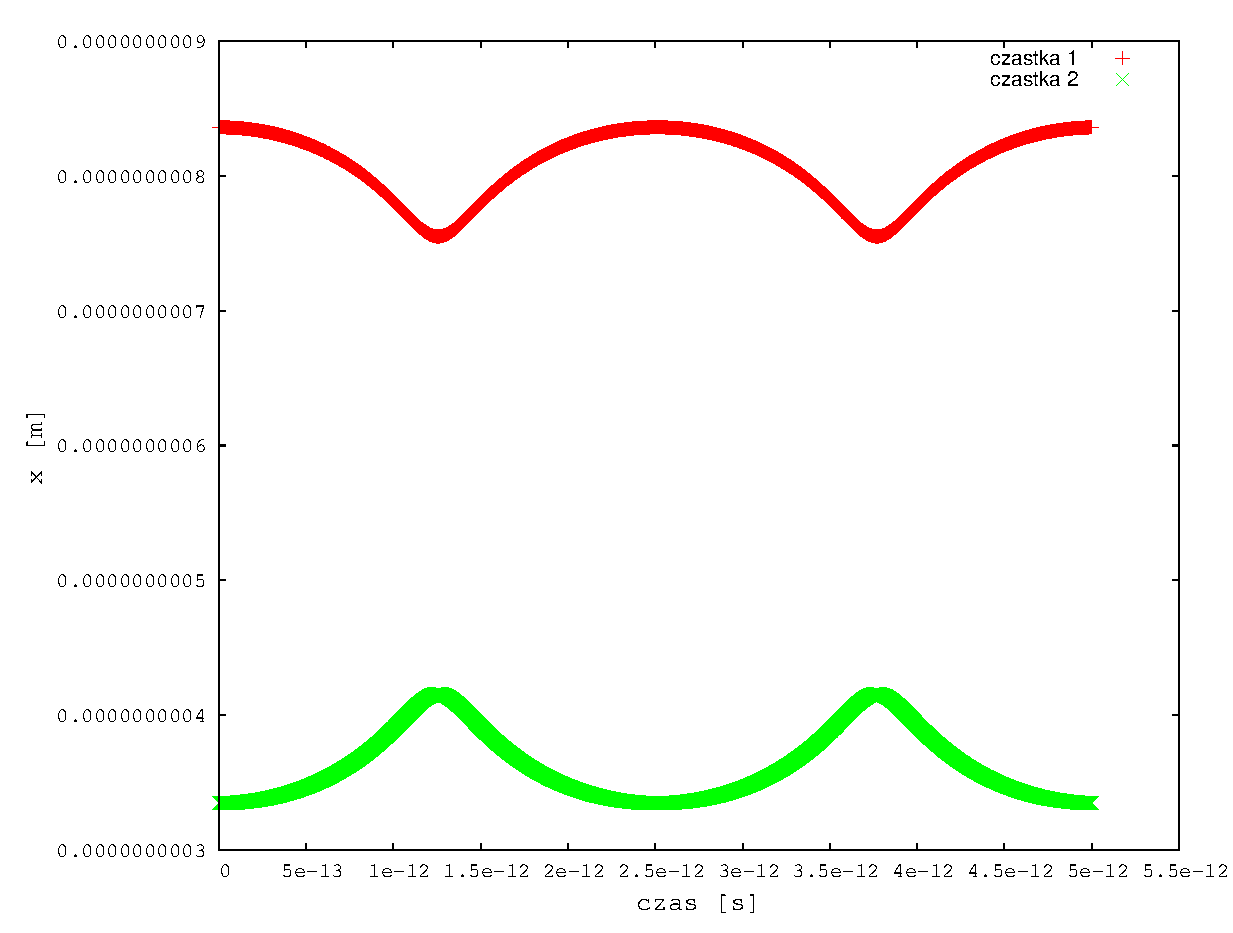
\includegraphics[scale=0.6]{wyniki/verlet-radius-in.eps}
\caption{Położenie cząstek w odległości promienia odcięcia}
\label{pic:verlet-radius-in}
\end{center}
\end{figure}
\FloatBarrier

\begin{figure}[h]
\begin{center}
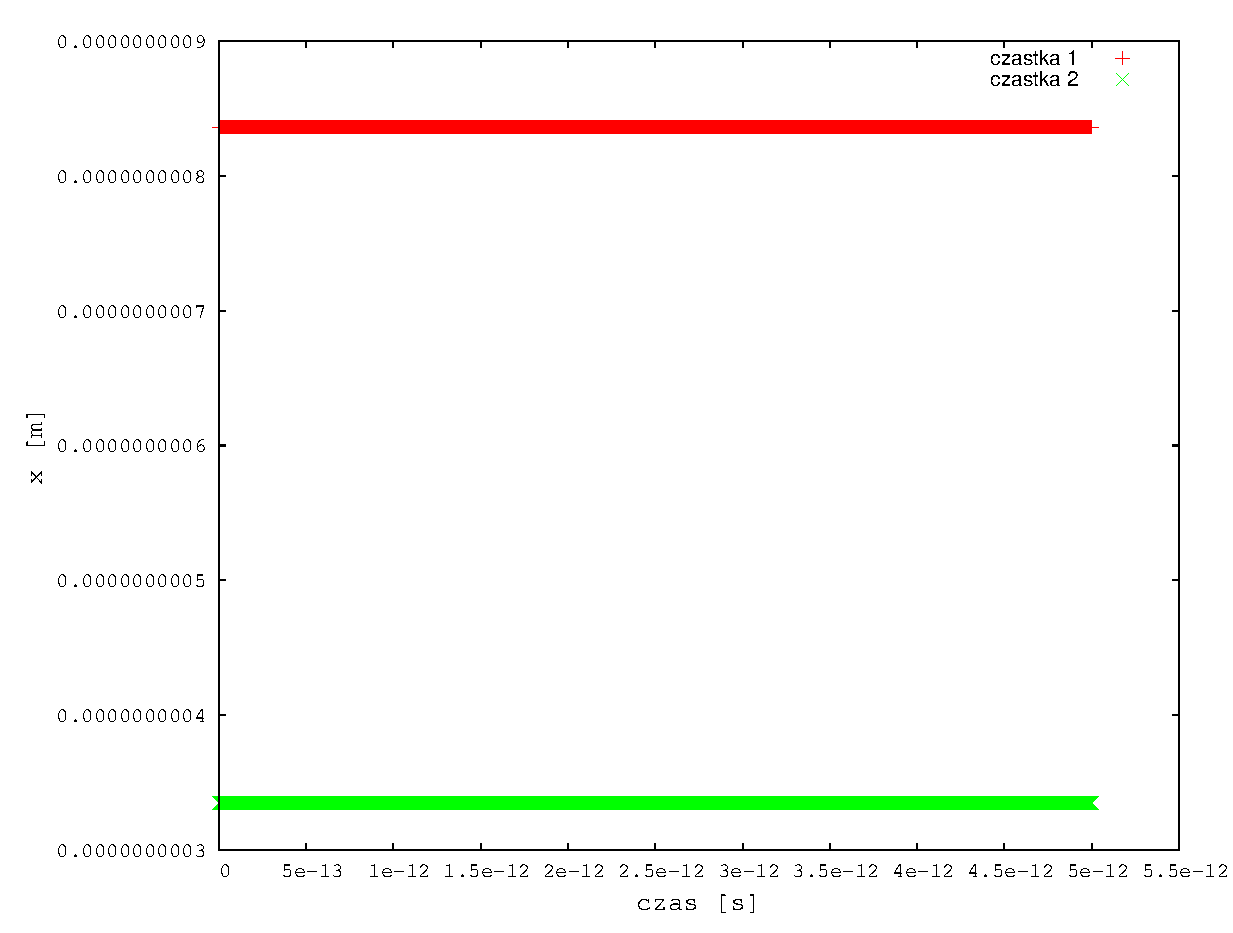
\includegraphics[scale=0.6]{wyniki/verlet-radius-out.eps}
\caption{Położenie cząstek w odległości większej niż promienia odcięcia}
\label{pic:verlet-radius-out}
\end{center}
\end{figure}
\FloatBarrier

W powyższych wykresów wywnioskować możemy, że promień odcięcia został prawidłowo zaimplementowany. W pierwszym przypadku odległość pomiędzy cząstkami nie przekraczała promienia odcięcia natomiast w drugim przypadku przekraczała.

\subsection{Symulacja dla wielu cząstek}

Symulacja gazu rzeczywistego została przeprowadzona dla $100$ cząstek w trójwymiarowym pudle obliczeniowym o wymiarach $10^{-8}m$ x $10^{-8}m$ x $10^{-8}m$. Został obrany krok czasowy $10^{-14}s$ natomiast całkowity czas symulacji $10^{-10}s$.

Cząstki układane są w pudle obliczeniowym równomiernie co pewien skok w każdym z wymiarów. Początkowa odległość pomiędzy cząstkami jest tak dobrana aby cząstki znajdowały się poza promieniem odcięcia każdej z cząstek. Dzięki temu na samym początku symulacji energia potencjalna wynosi 0 a z biegiem czasu wartość ta powinna oscylowć wokół zera. Prędkość początkowa dla każdej z cząstki losowana jest z rozkładu Maxwella o parametrach takich aby temperatura $500 K$ opisywała rozkład.

Poniżej przedstawiony został wykres poszczególnych składowych energii w funkcji czasu.

\begin{figure}[h]
\begin{center}
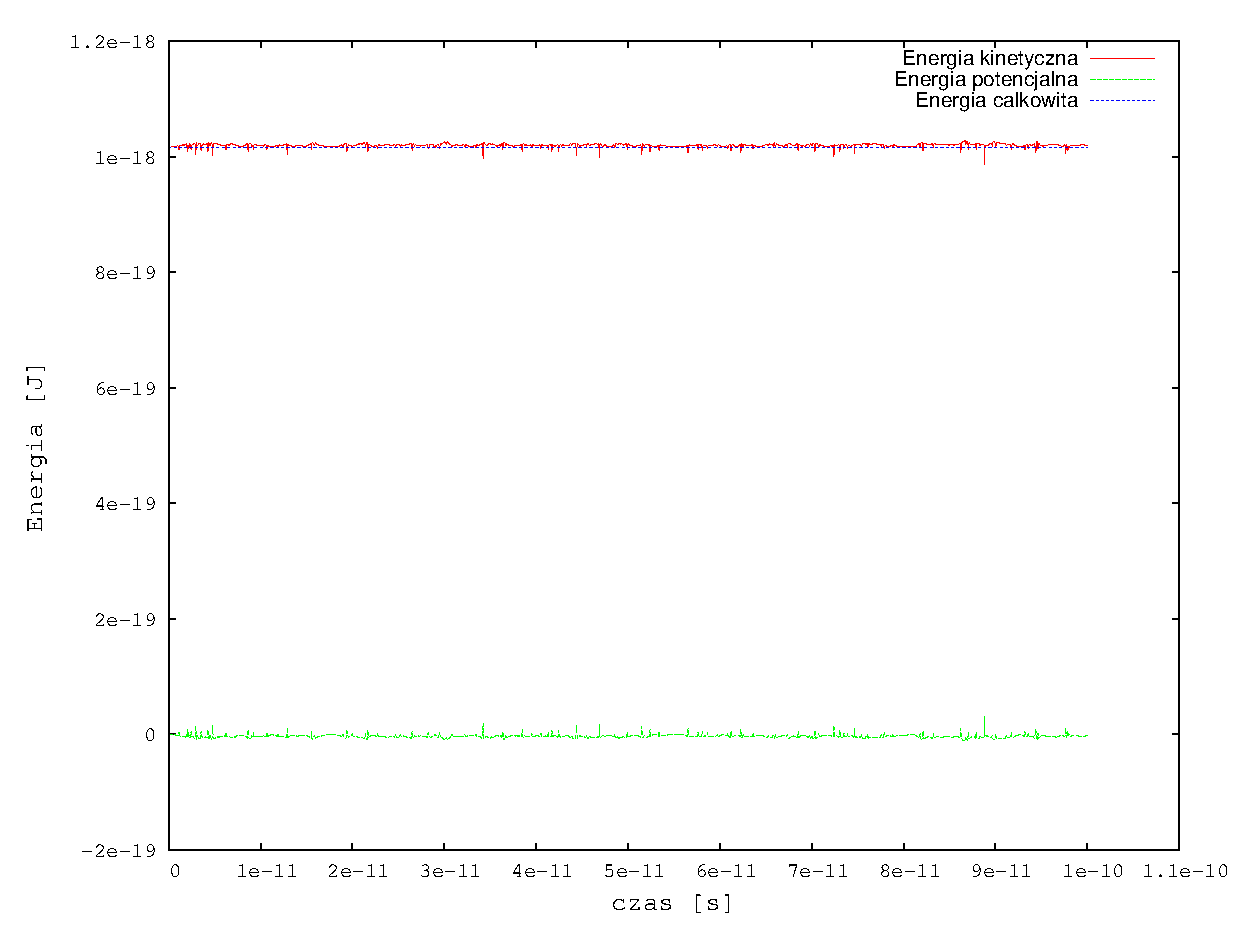
\includegraphics[scale=0.6]{wyniki/simulation.eps}
\caption{Energia 100 cząstek gazu znajdujących się w pudle obliczeniowym}
\label{pic:simulation}
\end{center}
\end{figure}
\FloatBarrier

Symulacja 100 cząstek została przeprowadzona bez żadnych problemów. Energia całkowita układu pozostaje stała. Każdy wzrost energii potencjalnej jest rekompensowany przez zmalenie energii kinetycznej i vice versa. Algorytm zachowuje się stabilnie dla obranego czasu trwania symulacji. Czas symulacji wynosił około $370$ sekund.

Sprawdzone zostały także parametry makroskopowe układu aby upewnić się, że model oraz symulacja jest poprawna.

\subsubsection{Temperatura gazu}

Aby wyznaczyć temperaturę za pomocą metod dynamiki molekularnej należy na początku obliczyć średnią energię kinetyczną cząstek. Następnie korzystając z twierdzenia o ekwipartycji energii można wyprowadzić wzór na bezprośrednią zależność temperatury od prędkości poszczególnych cząstek:

\begin{equation}\label{temp:1}
T = \frac{2}{3 k_B} \frac{1}{M N} \sum_{n=1}^{N} \sum_{m=1}^{M} \frac{m}{2} v_i^2(t_n)
\end{equation}

W przeprowadzonej symulacji temperatura badanego rzeczywistego gazu wynosiła $T=492.48K$.
Wartośc ta jest zbliżona do założonej wartości $500 K$. Należy pamiętać, że jest to jedynie wartość średnia i przy wielokrotnym uruchamianiu symulacji średnia temperatura gazu ze wszystkich symulacji dążyłaby do temperatury $500 K$.

Zbadane zostało także czy temepratura zmienia się wraz z czasem jej trwania.

\begin{figure}[h]
\begin{center}
\includegraphics[scale=0.6]{wyniki/simulation-temp.eps}
\caption{Temperatura gazu w funkcji czasu trwania symulacji}
\label{pic:simulation}
\end{center}
\end{figure}
\FloatBarrier

Początkowo temperatura gwałtownie rośnie czego autor nie jest w stanie racjonalnie wytłumaczyć. Aby zbadać ten efekt należałoby sprawdzić czy nie jest to przypadkiem spowodowane niezerowym krokiem czasowym bądź złym początkowym ustawieniem cząstek biorących udział w symulacji. Natomiast po niedługim czasie symulacja ulega ustabilizowaniu i temperatura z dokładnością do niedużych fluktuacji pozostaje stała co jest poprawne gdyż mamy do czynienia z odizolowanym układem.

\subsubsection{Ciśnienie gazu}

Do obliczenia ciśnienia gazu wykorzystany został sposób bazujący na mechanicznej definicji ciśnienia. Mianowicie ciśnienie jest to średni przekaz pędu na jednostkę powierzchni i jednostkę czasu na wybranej powierzchni $\Delta A$:

\begin{equation}\label{cisnienie:1}
p = m \frac{\Delta v_n^{sr}}{\Delta t \Delta A}
\end{equation}

gdzie: $\Delta v_n^{sr}$ jest uśrenioną po czasie zmianą prędkości prostopadłej do rozważanej powierzchni.
\\
\\
W przeprowadzonej symulacji ciśnienie badanego rzeczywistego gazu wynosiło $p=766877.44\ Pa$.

Zbadana została także zależność ciśnienia od czasu trwania symulacji.

\begin{figure}[h]
\begin{center}
\includegraphics[scale=0.6]{wyniki/simulation-cis.eps}
\caption{Ciśnienie gazu w funkcji czasu trwania symulacji}
\label{pic:simulation}
\end{center}
\end{figure}
\FloatBarrier

Należy podkreślić, że początkowe wartości ciśnienia są nieprawdziwie. Dopiero po odpowienim czasie możemy mówić o statystycznym przepływie cząstek przez odpowiednią ścianę pudła obliczeniowego. Po odpowednim czasie ciśnienie się stabilizuje i następują jedynie fluktuacje wynikające z tak małej ilości symulowanych cząstek oraz z niezerowego kroku czasowego.

\subsubsection{Równanie stanu gazu}

Do prostego sprawdzenia czy otrzymane wyniki nie są przekłamane sprawdzona została wartość ciśnienia jaka panowała by w pudle obliczeniowym przy zadanej temperaturze gdyby do gazu stosowało się równanie Clapeyrona (gaz doskonały) - co przy zadanej temperaturze jest dopuszczalnym uproszczeniem.

Zgodnie z równaniem Clapeyrona:

\begin{equation}\label{clap}
pV = NkT
\end{equation}

Obliczając ciśnienie przy temperaturze $T=492.48K$ otrzymujemy ciśnienie równe $p = 679969\ Pa$ co jest wartością bardzo zliżoną do wartości otrzymanej z symulacji. Pozwala to stwierdzić jakoby model oraz sposób przeprowadzania symulacji był prawidłowy.

%\begin{figure}[h]
%\begin{center}
%\includegraphics[scale=0.6]{output/energy.eps}
%\caption{Zależność błędu $E_c - E_{real}$ od czasu dla trzech wybranych kroków czasowych}
%\label{pic:energy}
%\end{center}
%\end{figure}
%\FloatBarrier

\section{Aplikacja}

\subsection{Kod źródłowy}
Oprogramowanie dostępne jest w publicznym repozytorium GitHub pod adresem\cite{repo}:

$$
https://github.com/KaRi94/MolecularDynamicsSimulator
$$

Aplikacja dostępna jest pod licencją MIT\cite{mit}.

\subsection{Opis kodu źródłowego}
Kod źródłowy posiada dokumentacje metod oraz użytych klas w formie docstringów. 

\subsection{Dalszy rozwój}
Oprogramowanie wymaga jeszcze dużo pracy aby mogło zostać użyte w naukowych celach. Autor sugeruje następujący dalszy rozwój aplikacji:

\begin{itemize}
\item Wielowątkowość w obliczeniach - w przypadku wielowątkowych komputerów kilkukrotny wzrost szybkości obliczeń
\item Zmiana implementacji metod odpowiedzialnych za obliczanie makroskopowych właściwości oraz energii potencjalej tak aby uwzględniały możliwość współistnienia w jednym pudle obliczeniowym gazów o różnych cząsteczkach/atomach.
\item Zmodularyzowanie klasy odpowiedzialnej za typ cząstki oraz rodzaj odziaływania tak aby ich zmiana nie wiązała się z ingerencją w kod źródłowy. Użytkownik mógłby załadować swoje typy cząstek/atomów.
\item Poprawa złożoności obliczeniowej (autor na czas dziesiejszy wie, że można obliczyć coś z lepszą złożonością wymaga to jednak zmian implementacyjnych)
\item Implementacja poprawki długozasięgowej
\end{itemize}


\section{Podsumowanie}
Podsumowując, problem badania gazu rzeczywistego za pomocą metod dynamiki molekularnej jest problemem niezwykle rozbudowanym. Obecna szybkość komputerów oraz superkomputerów nie jest wystarczająca abyśmy mogli symulować rzeczywisty gaz w którym mamy ok. $10^{23}$ cząsteczek. Najprawdopodopodobniej jeszcze przez wiele lat nie będziemy w stanie symulować ruch tak ogromnej ilości cząstek. Dlatego wykorzystane metody dynamiki molekularnej będą aktualne a ich ulepszanie oraz wiedza które aspekty można pominąć aby przyspieszyć proces symulacji będzie niezbędna do symulowania gazu rzeczywistego. Zbudowany model dobrze symuluje wiele aspektów cząstek poruszających się w zadanej objętości. Należy jednak podkreślić, że obecna aplikacja jest wolna i aby móc wykorzystywać ją do naukowych celów należałoby przebudować fragmenty kodu tak aby zyskać na złożoności obliczeniowej.

\newpage
\vfill
\begin{thebibliography}{9}
\bibitem{wikipedia}
    \url{https://pl.wikipedia.org/wiki/Algorytm_Verleta}
\bibitem{adamowski}
	\url{http://www.ftj.agh.edu.pl/~adamowski/wyklady_mofit_1/r9.pdf}
\bibitem{python}
    \url{https://www.python.org/}
\bibitem{gnuplot}
    \url{http://www.gnuplot.info/}
\bibitem{mit}
	\url{https://en.wikipedia.org/wiki/MIT_License}
\bibitem{repo}
	\url{https://github.com/KaRi94/MolecularDynamicsSimulator}

\end{thebibliography}

\end{document}
\grid
